% -*- coding: utf-8 -*-

\documentclass[b5paper,papersize,tombow,11pt]{jsbook}

\usepackage{amsmath,ascmac}
\usepackage{graphicx}
\usepackage{lettrine}
\usepackage{fancyhdr}
\usepackage{fancybox}
\usepackage{listings}
% Palatino
\usepackage{helvet}
\usepackage{euler}

%% Page Layout
% B5: 182mm x 257mm
\setlength{\voffset}{0mm}
\setlength{\topmargin}{-15mm}
\setlength{\textheight}{34\Cvs}
\setlength{\textwidth}{\fullwidth}
\setlength{\footskip}{10mm}

% set margin for openleft
% \setlength{\oddsidemargin}{-\oddsidemargin}
% \setlength{\evensidemargin}{-\oddsidemargin}


\pagestyle{fancy}

\fancyhead{}
% \fancyhead[RO,RE]{\rightmark}
% \fancyhead[LE,LO]{\leftmark}
\fancyhead[RO]{\rightmark}
\fancyhead[LE]{\leftmark}
\cfoot{\bfseries -- \thepage \ --} % page number at the center bottom
\renewcommand{\headrule}{
\vskip -1.5mm
\hskip-0.03\textwidth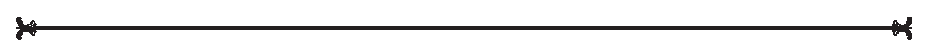
\includegraphics[width=1.06\textwidth,height=3.78mm]{images/hrule.eps}
\vskip -2.28mm
}

% jsbook.cls use 'plainhead' style for the first page of each chapter
\fancypagestyle{plainhead}{
\fancyhf{}
\cfoot{\bfseries -- \thepage \ --}
\renewcommand{\headrulewidth}{0.0pt}
\renewcommand{\headrule}{}
}

% jsbook.cls use 'empty' style for blank
\fancypagestyle{empty}{
\fancyhf{}
\cfoot{\bfseries -- \thepage \ --}
\renewcommand{\headrulewidth}{0.0pt}
\renewcommand{\headrule}{}
}

\makeatletter
\renewcommand{\chapter}{%
  \if@openright\cleardoublepage\else\clearpage\fi
  \plainifnotempty % 元: \thispagestyle{plain}
  \global\@topnum\z@
  \if@english \@afterindentfalse \else \@afterindenttrue \fi
  \secdef\@chapter\@schapter}
\def\@chapter[#1]#2{%
  \ifnum \c@secnumdepth >\m@ne
    \if@mainmatter
      \refstepcounter{chapter}%
      \typeout{\@chapapp\thechapter\@chappos}%
      \addcontentsline{toc}{chapter}%
        {\protect\numberline
        {\if@english\thechapter\else\@chapapp\thechapter\@chappos\fi}%
        #1}%
    \else\addcontentsline{toc}{chapter}{#1}\fi
  \else
    \addcontentsline{toc}{chapter}{#1}%
  \fi
  \chaptermark{#1}%
  \addtocontents{lof}{\protect\addvspace{10\p@}}%
  \addtocontents{lot}{\protect\addvspace{10\p@}}%
  \if@twocolumn
    \@topnewpage[\@makechapterhead{#2}]%
  \else
    \@makechapterhead{#2}%
    \@afterheading
  \fi}
\def\@schapter#1{%
  \chaptermark{#1}%
  \if@twocolumn
    \@topnewpage[\@makeschapterhead{#1}]%
  \else
    \@makeschapterhead{#1}\@afterheading
  \fi}

\def\@normalchapter[#1]#2{%
  \ifnum \c@secnumdepth >\m@ne
    \if@mainmatter
      \refstepcounter{chapter}%
      \typeout{\@chapapp\thechapter\@chappos}%
      \addcontentsline{toc}{chapter}%
        {\protect\numberline
        {\if@english\thechapter\else\@chapapp\thechapter\@chappos\fi}%
        #1}%
    \else\addcontentsline{toc}{chapter}{#1}\fi
  \else
    \addcontentsline{toc}{chapter}{#1}%
  \fi
  \chaptermark{#1}%
  \addtocontents{lof}{\protect\addvspace{10\p@}}%
  \addtocontents{lot}{\protect\addvspace{10\p@}}%
  \if@twocolumn
    \@topnewpage[\@makechapterhead{#2}]%
  \else
    \@makechapterhead{#2}%
    \@afterheading
  \fi}
\def\@normalschapter#1{%
  \chaptermark{#1}%
  \if@twocolumn
    \@topnewpage[\@makeschapterhead{#1}]%
  \else
    \@makeschapterhead{#1}\@afterheading
  \fi}
\def\@makechapterhead#1{%
  {\parindent \z@ \raggedright \normalfont
    \ifnum \c@secnumdepth >\m@ne
      \if@mainmatter
        \centering\huge\headfont \@chapapp\thechapter\@chappos
        \par\nobreak
        % \vskip \Cvs % 欧文は20pt
      \fi
    \fi
    \interlinepenalty\@M
    \begin{center}
     {\LARGE \headfont #1}\par\nobreak\noindent
\hskip-0.03\textwidth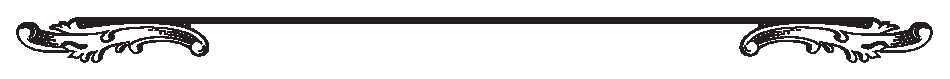
\includegraphics[width=1.06\textwidth,height=7.59mm]{images/chapter-title-ornament.eps}\vskip-7.59mm\vskip-0.5\Cvs
    \end{center}
    \par\nobreak
    \vskip 1.000\Cvs}} % 欧文は40pt
\def\@makeschapterhead#1{%
  {\parindent \z@ \raggedright
    \normalfont
    \interlinepenalty\@M
	\begin{center}
    {\LARGE \headfont #1}\par\nobreak\noindent
\hskip-0.03\textwidth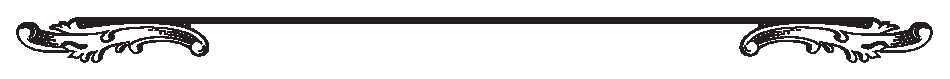
\includegraphics[width=1.06\textwidth,height=7.59mm]{images/chapter-title-ornament.eps}\vskip-7.59mm\vskip-0.5\Cvs
    \end{center}
	\par\nobreak
    \vskip 3\Cvs}} % 欧文は40pt

% section
% 後アキの調整
\renewcommand{\section}{%
  \if@slide\clearpage\fi
  \@startsection{section}{1}{\z@}%
  {\Cvs \@plus.5\Cdp \@minus.2\Cdp}% 前アキ
  {.7\Cvs \@plus.3\Cdp}% 後アキ
  {\normalfont\Large\headfont\raggedright}}

% 前・後アキの調整
\renewcommand{\subsection}{\@startsection{subsection}{2}{\z@}%
  {0.7\Cvs \@plus.5\Cdp \@minus.2\Cdp}% 前アキ
  {.25\Cvs \@plus.3\Cdp}% 後アキ
  {\normalfont\large\headfont}}


\makeatother

\renewcommand{\prechaptername}{}
\renewcommand{\postchaptername}{}

\makeatletter
\renewcommand{\thesection}{\S\,\@arabic\c@section}
\makeatother

\ifx\Cht\undefined
 \newdimen\Cht\newdimen\Cdp
 \setbox0\hbox{\char\jis2121}\Cht=\ht0\Cdp=\dp0\fi
\makeatletter
\long\def\linespace#1#2{\par\noindent
  \dimen@=\baselineskip\multiply\dimen@ #1\advance\dimen@-\baselineskip
  \advance\dimen@-\Cht\advance\dimen@\Cdp
  \setbox0\vbox{\noindent #2}\advance\dimen@\ht0\advance\dimen@-\dp0%
  \vtop to\z@{\hbox{\vrule width\z@ height\Cht depth\z@
   \raise-.5\dimen@\hbox{\box0}}\vss}%
  \dimen@=\baselineskip\multiply\dimen@ #1\advance\dimen@-\baselineskip
  \vskip\dimen@}
\makeatother

\title{The Database Times vol.2}
\date{2012/12/31}
\author{Hotchpotch Society}

\newcommand{\term}[2]{\noindent{\gt $\clubsuit$ #1}$\cdots$ #2}

%% Listings
\newcommand{\listingsize}{\small}
\lstset{language=SQL,
morekeywords={RETRIEVE,RANGE,OF,IS},
numbers = left,
numberstyle = {\tiny},
numbersep = 5pt,
breaklines = false,
breakindent = 40pt,
flexiblecolumns = true,
keepspaces = false,
basicstyle = \normalsize,
identifierstyle = \itshape\listingsize,
commentstyle = \fontfamily{ptm}\selectfont\listingsize,
stringstyle = \upshape\listingsize,
tabsize = 4,
escapechar = |,
}


\begin{document}

\thispagestyle{empty}

\frontmatter

% タイトルページ
\begin{center}
 
\includegraphics[width=10cm]{images/title.eps}
 \par\vspace*{50mm}
 \noindent Hotchpotch Society
\end{center}

% まえがきページ
% -*- coding: utf-8 -*-

\chapter*{まえがき}
\addcontentsline{toc}{chapter}{まえがき}
\thispagestyle{plainhead}


\begin{flushright}
 2012年 12月

Hotchpotch Society
\end{flushright}

\newpage

\subsection*{お品書き}

\noindent {\bf ■ データベースシステムの夜明け}

今の世の中,データベースシステムといえばリレーショナルデータベースシステムです。そのリレーショナルデータベースシステムが,一体どのようにして生み出されたのか,そしてどのように発展を遂げていったのか,その歴史を辿ります。

\thispagestyle{plainhead}


% 目次ページ
\setcounter{tocdepth}{0} % show only chapters
\tableofcontents

\mainmatter

\pagestyle{fancy}

% 本文ここから
% -*- coding: utf-8 -*-


\cleardoublepage
\plainifnotempty


\chapter{hoge}


\begin{flushright}
はやみず
\end{flushright}


hogehoge
% -*- coding: utf-8 -*-

% TODO: 読点句読点の置換
% TODO: タイトル考える
\chapter{IRRのおはなし}
% * (アスタリスク)付きの \chapter* コマンドは原則不可とする

\begin{flushright}
 {\headfont yuyarin} % ペンネーム
\end{flushright}

インターネットにおけるドメイン間ルーティングでは,運用の利便性やセキュリティの面から経路情報を管理するデータベースが求められている.
そこで使われるのがルーティングポリシーを記述することを目的としたIRR(Internet Routing Registry)というシステムである.
本稿ではIPルーティングの基礎を簡単に述べた後に,ドメイン間ルーティングの運用と経路ハイジャックの問題について述べ,IRRをの仕組みと現状を紹介する.

この記事ではIP通信の基礎(IPアドレスとサブネット,パケット転送の仕組み)に関する知識を有していることを前提とすることをご了承頂きたい.


% TODO: セクション区切りを考える
\section{AS間ルーティングと経路フィルタ}

\subsection{経路交換とルーティング}

% 図を書く?
IPネットワークの役割は宛先のノードまでIPパケットを届けることであるが,
宛先に対してパケットを届けるためには,どのルータにパケットを転送すればよいかを知る必要がある.
パソコンなどのエンドホストは出口になっているルータ(デフォルト・ゲートウェイ)にパケットをすべて送ればよいが,途中のルータはそうはいかない.
そのためにはルータ間で自分の到達可能な宛先ネットワークの情報を交換する.
経路を他のルータに伝えることを\textgt{経路広告}と呼び,お互いが広告し合う事で\textgt{経路交換}が行われる.

経路交換を行い,集められた経路情報からパケットを送信する経路を決定することを\textgt{ルーティング}と呼び,そのためのプロトコルを\textgt{ルーティングプロトコル}と呼ぶ.
ルーティングによって選ばれた経路はベストパスと呼ばれる.

経路は大きく分けて,\textgt{宛先ネットワーク},\textgt{ネクストホップ},\textgt{メトリック}の3つの情報で構成される.
宛先ネットワークは192.0.2.128/25のようにprefixで表現される.
ネクストホップは宛先ネットワークにパケットを送るために次にパケットを転送するノードのアドレスである.
メトリックは宛先ネットワークに対して複数のネクストホップがあった場合にどのネクストホップを優先するかを決めるための値である.
この値の内容はルーティングプロトコルによって異なる.

\subsection{ASとドメイン間ルーティング}

% 図を書く?
1つの同じポリシーで運用されるネットワークの範囲を\textgt{ドメイン}と呼ぶ.
また,このドメインを\textgt{AS(Autonomous System, 自律システム)}と呼び,4 byteの一意な番号である\textgt{AS番号}によって区別される.
なのでインターネットはASという自律的なネットワークが相互に接続した「ネットワークのネットワーク」ということができる.

ASの内部で行われるルーティングを\textgt{ドメイン内ルーティング(Intra-domain Routing)}と呼ぶ.
ドメイン内ルーティングは各ASで好きなように行うことができる.
日本ではOSPF,北米ではIS-ISが主なルーティングプロトコルとして利用されている.

ASの間で行われるルーティングは\textgt{ドメイン間ルーティング(Inter-domain Routing)}と呼ぶ.
ドメイン間ルーティングは全世界のすべてのASで共通のルーティングプロトコルを利用しなければならず,現在はBGP4が利用されている.
ドメイン間ルーティングではドメイン内のルーティングは隠蔽されている.

ある経路について経路広告を行なっている大元のASのことをOrigin ASと呼ぶ.

\subsection{AS間の接続関係}

インターネットはASが相互接続してできたネットワークであるという話をしたが,すべてのASが対等に接続しているわけではない.
AS間の関係には大きく分けて上下関係のトランジット(transit)と対等な関係のピア(peer)の2つが存在する.
このASの強弱関係は接続しているASの数や知っている経路の数,つまり到達性の広さで決まってくる.

トランジットはお金を支払って他のASから接続性を買う関係である.「トランジットを買う」とも言う.
接続性を売る側を親ASやトランジッタ,買う側を子ASやカスタマーなどと呼ぶ.
トランジットでは流れるトラフィック量に応じてMbps単価で月額料金が課金されることが多い.

ほとんどのASはトランジットを上位のASから購入している.どこからもトランジットを買わない最上位のASはTier 1と呼ばれる.
現在14のASがTier 1とされており,日本の事業者ではNTT CommunicationsのAS2914が唯一のTier 1である.

一方でピアは強弱関係の近いAS同士が無償で経路交換を行う関係である.
一般に「ピアを張る」と表現されるが,BGPにおける隣接関係をピアと呼ぶため,トランジットの関係でも技術的には「ピアを張る」ので文脈に注意する必要がある.
もともとトランジットを通して行われていたトラフィック交換をピアによって直接行うことにより,従量課金であるトランジットの使用料を下げることができる.

\subsection{経路広告とトラフィックコントロール}

さて経路広告を行うと,その経路宛のパケットが流れこんでくる.
正確には対向ASのルータにおいてルーティングのプロセスでベストパスに選ばれればである.

経路広告をしてもらうと,その経路宛のパケットが対向ASのルータに吸い込まれる.
自分ASのルータでベストパスに選ばれた対向ルータに吸い込まれるが,自分のASのルータなので制御は簡単である.

必要なトラフィックは自分のASを通して流しても良いが,自分に全く関係のないトラフィックであれば,
たとえお金のかからないピアであっても流したくないし,ましてやお金のかかるトランジットには死んでも流したくない.
平たく言えばタダ乗り禁止である.トラフィックが増えるほど設備が必要になるからだ.

そういった経済的な動機によって,トラフィックをコントロールしなければならないのだが,基本原則は存在する.
トランジットでは,親ASは子ASの広告する経路を全世界に対して広告する責任があり,子ASは親ASからの経路をすべて受け入れる.
ピアでは,自分の子ASと自ASの経路を広告し,ピア先のASとその子ASの広告する経路を受け入れる.
このへんの詳しい話は非常に面白いところだけれども,今回の本題からは逸れるのでまたの機会に.

トラフィックをコントロールする方法はいくつか存在するが,AS間においてはまず経路を広告するかしないかの二択である.
メトリックなどの細かいパラメータは経路を広告すると決めてからの話である.

\subsection{経路フィルタ}

どの相手にどの経路を広告するか,どの相手からのどの経路広告を受け入れるか,それを制御するためにルータに経路フィルタを設定する.
そのため,自ASが新しく経路広告を行うときは隣接ASにそれを伝えてフィルタを開けてもらわなければいけいない.
これにはメールが使われていることが多いが,隣接ASが自ASの経路を広告している場合は,さらにその隣接ASにもフィルタを空けてもらう必要がある.
このようなケースはトランジットで起こりうるのだが,最上位のTier 1の労力は半端なものではない.
AS RankによればAS2914は全世界の約1/3の13,242の子ASを抱えて156,530のIPv4の経路を広告している.
人手のかかるメールなんかではやってられないので,経路情報をデータベース化して自動的にフィルタを生成して反映される仕組みが必要になってくる.

\section{資源管理と経路ハイジャック}

\subsection{AS番号とIPアドレスの関係}

インターネットは自律的なシステムではあるが,AS番号やIPアドレスなどの資源は重複利用が生じないように誰かが統一的に管理を行わなければならない.
こういった資源は階層的に組織されたInternet Registryによって管理されていて,
日本の場合では,最上位のIANA,アジア太平洋地域のAPNIC,日本国のJPNICのようにして階層的に資源が割り当てられている.
ちなみに欧州地域はRIPE,北米地域はARINで,日本におけるAPNICに相当する.
日本国内でAS番号やIPアドレスを取得する場合はJPNICを窓口として割り振りを受ける.

AS番号もIPアドレスもそれぞれが取得を申請した組織や個人に割り振られるため,AS番号とIPアドレスは資源管理上は直接の関係性を持っていない.
また,一つの組織が複数のASを運用することも多いし,他の組織の子ASにアドレスブロックを貸与することもあるため,
実際にどのASからどの経路が広告されるかは,広告されてみないとわからない.
もちろんネットワークの運用者は自分のASから広告する経路を知っているが,他のASのことはわからない.

\subsection{経路ハイジャック}

JPNICのような組織からまだ割り振りを受けていないアドレスブロックや,
他の組織が取得しているアドレスブロックを勝手に広告することは技術的には可能である.
単純にルータにそういう設定を入れればいいだけで,免許のようなものはいらない.
こういう事例を経路ハイジャックと呼ぶ.

前章で経路を流すとトラフィックが流れることを説明した通り,経路ハイジャックを受けると,
本来自分のASに流れるはずだったトラフィックが他のASに流れてしまう.
パケットが到達不能で破棄される可能性や,盗聴・改竄の恐れもある.

経路ハイジャックは頻繁に起きていて,そのほとんどはアドレスの打ち間違いやAS外に出さない経路を漏らしてしまうなどの設定ミスである.
大規模な事件としてはパキスタンテレコムがYouTubeの経路をハイジャックしてしまい,YouTubeにアクセス不能になった事件などが挙げられる.
この事件ではパキスタン国内でYouTubeへのアクセスを遮断するために偽の経路情報を流してトラフィックを吸い込もうとしたところ
設定ミスで偽の経路情報をAS外部に漏らしてしまったのが原因だと言われている.

こうした経路ハイジャックが行われた際に,すぐに気づくことが出来る仕組みが必要になる.
経路ハイジャックかどうかを調べるためには,その経路のOrigin ASが妥当であるかを見ればいいのだが,
前述のとおりASとIPアドレスの対応表なんてものはないため,調べることはできない.

根本的な解決として署名付きの経路を流すBGPsecなどが提案されているが,
ひとまずの運用的な対処として,Origin ASと経路の関係性の情報を持ったデータベースを作成して,
それとBGPで実際に流れている経路を比較することで,ハイジャックを検知する取り組みが行われている.
そのためには当然,正確なOrigin ASと経路の関係性の情報を持ったデータベースが必要になる.

\section{IRR}

\subsection{IRRとは何か}

さて,ここまで経路フィルタの自動生成という運用上の問題と経路ハイジャックの検知という2つの目的から,
経路に関連する情報を持ったデータベースが必要になっているという話をした.
そこで登場するのがIRR(Internet Routing Registry)である.
名前の通り,インターネットのルーティング情報を登録するシステムで,
もともとは高度なルーティングポリシーを記述でき,その運用者の情報なども管理できるものである.

歴史を少し述べると,IRRは,1980年代のNSFNetの時代にコンフィグを自動生成するための,高レベルなルーティングポリシーを記述するためのデータベース(PRDB)から由来している.
その後,1989年にRIPEの最初のミーティングが行われ,1994年にRIPE-181という文書で現在使われているオブジェクトクラスベースの構造の概念が導入され,1995年にIETFにてRFC1786として標準化さた.
最終的に1999年にRFC2622 Routing Policy Specification Language (RPSL)として標準化されRFC4012でIPv6用の拡張が行われ現在に至っている.

IRRではwhoisをプロトコルに使っているためwhoisコマンドを用いて利用することができる.
実装はRIPE NCCのRIPE DB ServerとMeritのIRRdの2つがメジャーである.

\begin{quote}
\begin{verbatim}
$ whois -h jpirr.nic.ad.jp AS4713
\end{verbatim}
\end{quote}

\newenvironment{minilinespace}{
\baselineskip = 4mm
}

\begin{tabular}{l}
\begin{itembox}[c]{aut-numオブジェクト}
\begin{quote}
\begin{minilinespace}
\begin{verbatim}
% whois -h whois.radb.net AS2500 
aut-num: AS2500
as-name: WIDE
descr:   WIDE Project in Japan
admin-c: JM46-AP
tech-c:  AK27-AP
import:  from AS-NSPIXP2
           action pref=100;
           accept ANY
import:  from AS2501
           action pref=100;
           accept AS2501 AS7531                     
(snip)
export:  to AS-NSPIXP2 announce AS112 AS2500 AS2501 (snip) AS55384
export:  to AS2504 announce ANY and NOT AS7660      
(snip)
notify:  two@wide.ad.jp
mnt-by:  MAINT-AS2500
changed: kato@wide.ad.jp 20121024
source:  RADB
\end{verbatim}
\end{minilinespace}
\end{quote}
\end{itembox}
\\
\begin{itembox}[c]{routeオブジェクト}
\begin{quote}
\begin{minilinespace}
\begin{verbatim}
% whois -h whois.radb.net 1.1.1.1
route:   1.1.1.0/24
descr:   Google
origin:  AS15169
notify:  radb-contact@google.com
mnt-by:  MAINT-AS15169
changed: radb-contact@google.com 20121119
source:  RADB
\end{verbatim}
\end{minilinespace}
\end{quote}
\end{itembox}
\\
\begin{itembox}[c]{as-setオブジェクト}
\begin{quote}
\begin{minilinespace}
\begin{verbatim}
% whois -h jpirr.nic.ad.jp AS-OCN
as-set:  AS-OCN
descr:   ASes advertised by OCN
members: AS4713,
         AS290,   AS1628,  AS2499,  AS2506,  AS2509,
         AS2515,  AS2518,  AS2526,  AS4680,  AS4683,
         (55 lines snipped)
         AS131154, AS131154, AS131155, AS132095, AS132119
admin-c: Ichiro Mizukoshi
tech-c:  Tomoya Yoshida
notify:  admin@ocn.ad.jp
mnt-by:  MAINT-AS4713
changed: admin@ocn.ad.jp 20121206
source:  JPIRR
\end{verbatim}
\end{minilinespace}
\end{quote}
\end{itembox}

\end{tabular}

\subsection{IRRの構造}

IRRにはいくつかの種類のクラスが定義されていて,それらをオブジェクトとして登録していくことで成り立っている.
RFC2622/4012では,
route, route6, aut-num, as-set, route-set filter-set rtr-set peering-set inet-rtr, mntner, role, person
といったクラスが定義されている.このうち今回は特によく利用されているaut-num, route, as-setについて紹介する.
百聞は一見にしかずなので登録されているデータを見て頂きたい.

\subsubsection{aut-numクラス}
aut-numクラスはASを表現したクラスでASという接頭辞の後にAS番号を続けたものをキーに使う.
大体の属性値は見ていただければわかると思うが,特筆したいのが,export/import属性である.
この属性には肝心要のルーティングポリシーを記述することができる.
importの例では,AS-NSPIXP2(これは後述のAS-SETオブジェクト)に含まれるASから広告されるに対して,
経路のpreferenceを100にしながらすべての経路を受け入れるというポリシーを記述している.
一方でAS2501からの経路に対してはAS2501とAS7531の2つのASがOriginである経路しか受け入れない.
exportの例ではAS2504に対してAS7660を除くすべての経路を広告するというポリシーを記述している.

この例はAS2500のWIDE Projectという日本の研究機関のASのものであるが,
先に述べたようにASの接続関係は接続性の売り買いの話につながるため,
ポリシーがオープンなコンテンツプロバイダや研究機関を除いた商用のISPなどで,
ここまで細かく記述されていることは滅多に見かけない.

\subsubsection{routeクラス}
routeクラスは経路情報を表現したクラスで,広告されるプレフィックスをroute属性に使う.
IPv6の経路はroute6クラスで表現される.
origin属性にはその経路を広告するASのaut-numオブジェクトが書かれていて,routeとoriginを合わせてこのオブジェクトのキーとしている.
そのため1つの経路に対して複数のoriginが存在することもある.
運用上複数のOrigin ASから同一の経路を広告する可能性があるため,そのようになっている.

\subsubsection{as-setクラス}
as-setクラスはaut-numオブジェクトの集合体を表現したクラスで,AS-という接頭辞の後に名称を続けたものをキーに使う.
例はAS-OCNというNTT CommunicationsのOCN(AS4713)のas-setである.
このASは国内のトランジット事業者でもあるので多くの子ASを抱えており,その経路を上位のトランジットに対して広告する必要がある.
その際にAS4713の子ASが誰であるかを上位ASはいちいち気にしたくないので,as-setとしてまとめて教えてあげている.

\subsubsection{mnt-by属性とsource属性}
これらのクラスに共通して存在する属性の中にmnt-by属性とsource属性がある.
mnt-by属性はそのオブジェクトを管理している組織を示す属性で,mntnerクラスのオブジェクトが登録される.
mntnrクラスのオブジェクトにはパスワードが設定できるため,mnt-by属性を指定することで他者からのデータの上書きを防ぐことができる.
source属性はそのオブジェクトがどのIRRに登録されたものかを示している.
後述するがIRRは複数の組織で独立して運用されていて,それらの間でデータを同期している.
問い合わせを行うIRRホストと,オリジナルのオブジェクトが登録されているIRRホストは別になるため,この属性が必要になる.

\subsection{IRRの運用}

IRRは世界の30以上の組織でそれぞれ運用されている.
APNICやJPNIC,RIPEなどのInternet Registryが運用するもの,NTT CommunicationsやLevel3などのISPが運用するもの,Meritなど研究機関が運用するものに分類することができる.
日本から使う場合はJPNICのJPIRR,MeritのRADB(Routing Assets Database),NTT CommunicationsのNTTCOMが有名である.

これらのIRRはデータベースを他のIRRと同期しているが,組織の関係によっては同期していないこともある.
例えば研究機関であるMeritの運用するRADBはほとんどのIRRのミラーを行なっている.
NTTCOMはJPNICのJPIRRをミラーしているが,JPIRRはNTTCOMをミラーしていない.
これは公的機関が一営利企業のミラーを行うということに対する大人の事情でそうなっている.

\subsection{IRRが必要とされる場面}

IRRは任意加入のデータベースだが,利用を迫られる時がある.
基本的には経路フィルタの自動生成を行うためにIRRが使われる.

例えばNTTCOMやLEVEL3のようなTier1トランジット(ISPのためのISP)では経路フィルタ適用などの運用を簡略化するために,
顧客に対して自身のIRRに経路情報を登録することを求めている\footnote{http://www.us.ntt.net/support/policy/rr.cfm}.
また同様の理由で他のASに対してピアを張るための条件としてIRRの登録を求めるASも存在する.
他にもIX(Internet Exchange)でroute serverを使ってmulti lateral peeringを行う際の経路フィルタの登録などにも利用される.

フィルタの生成の他には経路情報からコンタクトパーソンを見つけるためや,
障害時のトポロジー把握などに使われる.

\subsection{IRRの歩き方}

ではそろそろ手を動かしたくなって疼いてきた頃だと思うので,一般のご家庭でよく使われるIRRの使い方を紹介しよう.

origin ASを指定して経路の一覧を取得するときは!gを使う.
UNIXの場合は!を\verb+\+でエスケープする必要がある.
メモリ管理が必要な古のプログラムからでも読みやすいように整形されて表示され,Aはデータの長さ,Cは終了を意味している.

\begin{quote}
\begin{minilinespace}
\begin{verbatim}
% whois -m \!gAS7521
A116
210.173.160.0/19 210.173.176.0/24 210.173.178.0/25 218.100.45.0/24 (snip)
C
\end{verbatim}
\end{minilinespace}
\end{quote}

AS-SETをASの一覧に展開したいときは!iオプションを使う.AS-SETの中にAS-SETが含まれるような場合は,1をつけてAS-SETの再帰展開を行う.

\begin{quote}
\begin{minilinespace}
\begin{verbatim}
% whois -m \!iAS-GOOGLE,1 
A126
AS11344 AS13949 AS1424 AS15169 AS19425 AS22577 AS26910 AS36040 (snip)
C
\end{verbatim}
\end{minilinespace}
\end{quote}

AS7521がメンテナになっているオブジェクトを列挙する.だいたいこのあとに属性でgrepをかける.

\begin{quote}
\begin{minilinespace}
\begin{verbatim}
% whois -m \!oMAINT-AS7521 
A10130
route:      210.173.160.0/19
descr:      INTERNET MULTIFEED CO.
(snip)
source:     JPIRR
C
\end{verbatim}
\end{minilinespace}
\end{quote}

AS7521の情報でsourceがJPIRRのものだけを選択する.sourceによっては情報が間違っていたりすることがあるので,
情報の信頼性の高いsourceを指定したくなる場合がある.
ダブルクオーテーションで囲ってwhoisのオプションに間違われないようにする.

\begin{quote}
\begin{minilinespace}
\begin{verbatim}
% whois -h jpirr.nic.ad.jp -- "-s JPIRR AS7521"
aut-num:    AS7521
as-name:    MFEED
(snip)
source:     JPIRR
\end{verbatim}
\end{minilinespace}
\end{quote}

\subsection{もっと楽しいIRRの使い方}

ISC(Internet Systems Consortium)が開発しているIRRToolSet\footnote{http://www.isc.org/software/irrtoolset}を使うことでもっと快適なIRR生活を送ることができる.

pevalはIRR用にwhoisをもっと簡単にしたものである.as-ocn and as-iijのような記述をすればOCNとIIJの両方から広告されているプレフィックスの一覧
(OCNとIIJでマルチホーム接続しているASの経路)を取得することができる.

\begin{quote}
\begin{minilinespace}
\begin{verbatim}
peval "as-ocn"
({223.223.164.0/24, 223.223.165.0/24, 223.223.166.0/24, ... })
peval "as-ocn and as-iij"
src/peval/peval "as-ocn and as-iij"
({223.223.160.0/22, 223.223.0.0/17, 223.29.244.0/22, ...})
\end{verbatim}
\end{minilinespace}
\end{quote}

RtConfigはCiscoやJuniperのルータ用のフィルタやstatic routeを生成することができるツールである.

\begin{quote}
\begin{minilinespace}
\begin{verbatim}
% rtconfig -cisco_use_prefix_lists
rtconfig> @RtConfig access_list filter AS15169
!
no ip prefix-list pl100
ip prefix-list pl100 permit 1.0.0.0/24
ip prefix-list pl100 permit 1.1.1.0/24
ip prefix-list pl100 permit 1.2.3.0/24
ip prefix-list pl100 permit 8.8.4.0/24
ip prefix-list pl100 permit 8.8.8.0/24
ip prefix-list pl100 permit 8.34.208.0/20 ge 21 le 21
ip prefix-list pl100 permit 8.34.208.0/20 ge 23 le 24
(snip)
ip prefix-list pl100 deny 0.0.0.0/0 le 32

% rtconfig -config junos
rtconfig> @RtConfig access_list filter AS290
policy-statement prefix-list-100 {
  term prefixes {
    from {
      route-filter 45.1.0.0/16 exact accept;
      route-filter 130.128.0.0/15 prefix-length-range /16-/16 accept;
      route-filter 202.17.221.0/24 exact accept;
    }
  }
  term catch-rest {
    then reject;
  }
}
\end{verbatim}
\end{minilinespace}
\end{quote}

\section{IRRの問題}



% 本文ここまで

\cleardoublepage
\plainifnotempty
\refstepcounter{chapter}
\addcontentsline{toc}{chapter}
{\protect 雑談}
\chaptermark{雑談}

\begin{center}
 
\includegraphics[width=3cm]{images/zatsudan.eps}
\end{center}

\footnotesize

% -*- coding: utf-8 -*-

% 雑談ページ
%
% (<名前>) <内容> のフォーマットで各自適当なことを書くべし
%

\begin{itemize}
 \item (はやみず) 博士課程だけどコミケさえあれば関係ないよねっ
 \item (すーじー) 社二病でもニートがしたい!
 \item (ぜんぶつ) インフラエンジニアでも恋がしたい!
 \item (ゆやりん) 脇腹強打したのでこれから骨が折れてないか診てもらいに病院に行く
\end{itemize}


\normalsize

\newpage

\plainifnotempty

\section*{著者紹介}

\noindent {\gt ■ はやみず} \quad
某研究施設にて、データベースシステムと戯れる日々を過ごしている。昔はLisp系
言語に傾倒したり、マルチコア向け並列処理フレームワークの研究をしたりして
いた。この本の首謀者。

\vspace*{60mm}

% 奥付
\begin{center}
 
\includegraphics[width=8cm]{images/colophon.eps}
 \par\vspace*{1mm}
 \begin{tabular}{rl}
  \hline
  タイトル & The Database Times vol.2 \\
  発行日 & 2012年12月31日 初版発行 \\
  サークル & Hotchpotch Society \\
  著者 & はやみず、(TODO: to be updated) \\
  表紙デザイン & Eliza \\
  連絡先 & {\it yuto+c83@hayamiz.com} \\
  ウェブサイト & {\it http://hayamiz.com/\~{}hotchpotch/} \\
  印刷所 & TODO: \\
  \hline
 \end{tabular}
\end{center}

\end{document}
